% Source printed pp. 32-35, entire Section 1.5.
\section{为何使用平展拓扑?}\label{src:1.5}
\begin{epigraph}
可以说, 从 Zariski 拓扑转到平展拓扑时, 对于一个有限常值系数群 $G$, 为了得到``正确的'' $H^1$, 我们已经``做了该做的事''...一个值得注意的事实是, 这也足以对任意挠系数群找到``正确的'' $H^i(X,G)$(至少当 $G$ 与 $X$ 的剩余特征互素时). 这将在本讨论班的后续部分证明.
\epigraphauthor{Alexander Grothendieck~\cite[VII.2.1]{SGA4}}
\end{epigraph}
下一节将通过结合模函子与群胚来引入模叠: 需要指定每个概形 $S$ 上的对象族, 以及它们之间的等同和拉回. 为使这些数据定义一个\textit{叠}, 我们将要求对象及其态射在\textit{平展}拓扑中能够粘合!据说, Grothendieck 创造``étale''一词, 是因为平展态射使他联想到满月下涨潮时平静的海面, 正如 Victor Hugo 在``海上劳工''中写道: ``海面平静, 但退潮已开始显现.''

为何 Zariski 拓扑不足以满足我们的需要?简短的回答是: Zariski 开子集不够多, 而平展态射可以很好地替代解析开子集.

\subsection{平展态射究竟是什么?}\label{src:1.5.1-subsection}
有时我会感到困惑: 一个学生竟会被平展态射吓住, 尤其是当她已经掌握了概念上更困难的固有性, 平坦性等概念时. 一个原因可能是, 这一定义埋藏在~\cite[习题 III.10.3--6]{Har77}~中, 那里并未突出它的重要性.
% The supplied draft has no numbered object 1.5.1. It prints 1.5.2
% both beside the illustration and in its caption; retain both occurrences.
\setcounter{theorem}{1}
\begin{figure}[htbp]
\centering
\begin{minipage}[c]{.26\textwidth}
\centering
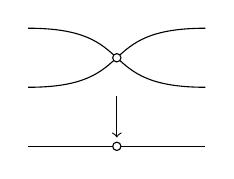
\begin{tikzpicture}[x=.75cm,y=.75cm,baseline=(current bounding box.center)]
\draw (-1.5,2)..controls (.4,2) and (-.4,1)..(1.5,1);
\draw (-1.5,1)..controls (.4,1) and (-.4,2)..(1.5,2);
\filldraw[fill=white] (0,1.5) circle (1.5pt);
\draw[->] (0,.85)--(0,.15);
\draw (-1.5,0)--(1.5,0);
\filldraw[fill=white] (0,0) circle (1.5pt);
\end{tikzpicture}
\end{minipage}\hfill
\begin{minipage}[c]{.16\textwidth}
\centering
$\begin{tikzcd}[row sep=large,column sep=small]
\mathbb A^1\arrow[d] & x\arrow[d,mapsto]\\
\mathbb A^1 & x^2
\end{tikzcd}$
\end{minipage}\hfill
\begin{minipage}[c]{.30\textwidth}
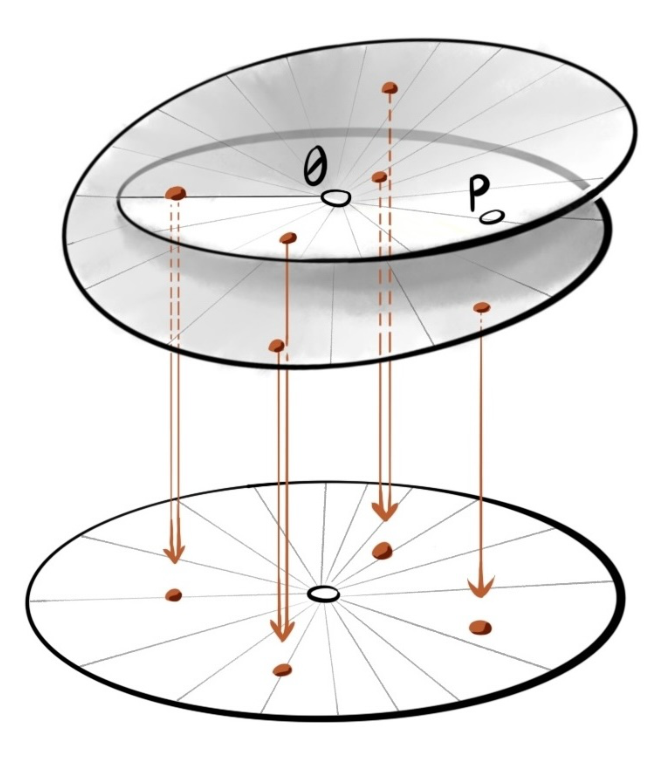
\includegraphics[width=\linewidth]{figures/fig-1.5.2-complex.png}
\end{minipage}\hfill
\begin{minipage}[c]{.12\textwidth}
\raggedleft(\ref{src:1.5.2})
\end{minipage}
\caption{$\mathbb A^1\setminus0$ 的平展二重覆盖. 左图画在 $\mathbb R$ 上(不过, 我们仍将负数的两个平方根画了出来), 右图画在 $\mathbb C$ 上.}\label{src:1.5.2}
\end{figure}
心中应有的几何图像是一个覆盖空间. 对 $\mathbb C$ 上有限型概形之间的态射 $f:X\to Y$, 平展性可以用以下几种方式表述: 
\begin{itemize}
\item $f$ 光滑且相对维数为 $0$(即 $f$ 平坦, 且所有纤维都光滑, 维数为 $0$); 
\item $f$ 平坦且非分歧(即对所有 $y\in Y(\mathbb C)$, 概形论纤维 $X_y$ 同构于点的不交并 $\coprod_i\operatorname{Spec}\mathbb C$); 
\item $f$ 平坦且 $\Omega_{X/Y}=0$; 
\item 对所有 $x\in X(\mathbb C)$, 在完备化上诱导的映射 $\widehat{\mathcal O}_{Y,f(x)}\to\widehat{\mathcal O}_{X,x}$ 为同构; 以及
\item 若还假设 $X$ 和 $Y$ 光滑, 则对所有 $x\in X(\mathbb C)$, 在切空间上诱导的映射 $T_{X,x}\to T_{Y,f(x)}$ 为同构.
\end{itemize}
若存在 $x\in X$ 的开邻域 $U$, 使 $f|_U$ 平展, 则称 $f$ \textit{在 $x$ 处平展}. 更多背景见 \S\bookref{A.3}. 这些刻画都彼此等价, 但绝不应认为你理当看出这一点: 有些证明相当复杂. 不过, 若暂且接受这些等价性, 那么只须很少的努力, 就不但能理解这一概念, 还能掌握它的运用.
\begin{exercise}[适于练习]\label{src:1.5.3}
证明 $f:\mathbb A^1\to\mathbb A^1$, $x\mapsto x^2$ 在 $\mathbb A^1\setminus0$ 上平展, 但在原点处不平展. 尝试尽可能多地使用上述刻画来证明.
\end{exercise}

\subsection{在平展拓扑中能看到什么?}\label{src:1.5.2-subsection}
使用平展拓扑, 就像给你的代数几何眼镜加上一副放大镜, 使你能看清那些通过微分几何眼镜早已能观察到的精细结构.
\begin{example}[结点的可约性]\label{src:1.5.4}
考虑平面中由 $y^2=x^2(x-1)$ 定义的平面结点三次曲线 $C$. 结点 $p=(0,0)$ 有一个可约的解析开邻域, 却没有这样的 Zariski 开邻域. 然而, 取 $x-1$ 的``平方根'', 就得到一个可约的平展邻域. 更具体地, 定义
$C'=\operatorname{Spec}\mathbb C[x,y,t]_t/(y^2-x^3+x^2,t^2-x+1)$, 并考虑
\[
C'\longrightarrow C,\qquad(x,y,t)\longmapsto(x,y).
\]
由于 $y^2-x^3+x^2=(y-xt)(y+xt)$, 可见 $C'$ 可约. 下图说明了这一点, 此图也见于~\cite[习题 III.10.6]{Har77}.
\end{example}
\begin{figure}[htbp]
\centering
\begin{tikzpicture}
\node[anchor=south west,inner sep=0] (art) at (0,0) {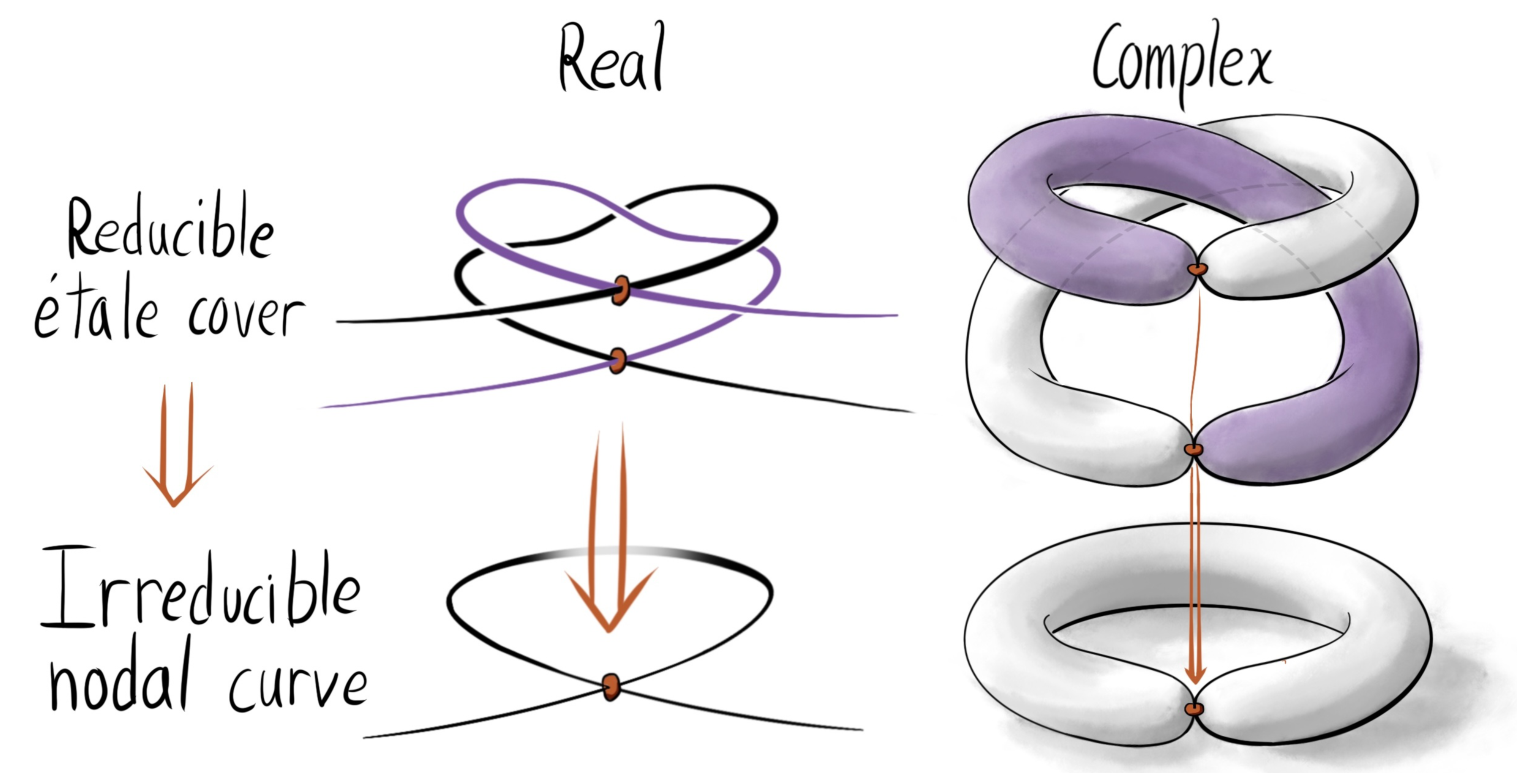
\includegraphics[width=.70\textwidth]{figures/fig-1.5.5.png}};
\begin{scope}[x={(art.south east)},y={(art.north west)}]
\fill[white] (.31,.88) rectangle (.44,1);
\node[font=\small] at (.375,.945) {实情形};
\fill[white] (.66,.85) rectangle (.86,1);
\node[font=\small] at (.76,.945) {复情形};
\fill[white] (.005,.535) rectangle (.215,.78);
\node[font=\scriptsize,align=center] at (.115,.67) {可约的\\平展覆盖};
\fill[white] (.012,.075) rectangle (.245,.31);
\node[font=\scriptsize,align=center] at (.13,.18) {不可约的\\结点曲线};
\end{scope}
\end{tikzpicture}
\caption{经过平展覆盖后, 结点三次曲线变得可约.}\label{src:1.5.5}
\end{figure}
\begin{example}[平展上同调]\label{src:1.5.6}
Zariski 拓扑中的层上同调可以推广到平展拓扑, 得到极为强大的\newterm{平展上同调}{étale cohomology}理论. 例如, 对 $\mathbb C$ 上亏格为 $g$ 的光滑射影曲线 $C$, 有限常值层 $\mathbb Z/n$ 的平展上同调 $H^1(C_{\text{ét}},\mathbb Z/n)$ 同构于 $(\mathbb Z/n)^{2g}$, 正如通常的上同调群一样; 而 Zariski 拓扑中的层上同调 $H^1(C,\mathbb Z/n)$ 为 $0$. 最后, 如果不提及平展上同调在证明 Weil 猜想方面的惊人应用, 那就有所疏漏了.
\end{example}
\begin{example}[平展基本群]\label{src:1.5.7}
你是否想过, Galois 理论中间域扩张与 Galois 群的子群之间的双射, 与代数拓扑中覆盖空间与基本群的子群之间的双射, 有某种相似之处?那么你并不孤单: Grothendieck 也考虑过这一点, 并发展出优美的\newterm{平展基本群}{étale fundamental group}理论, 将 Galois 群和基本群纳入同一框架.
\end{example}
\begin{example}[有限群自由作用的商]\label{src:1.5.8}
若有限群 $G$ 在射影簇 $X$ 上自由作用, 则商 $X/G$ 作为射影簇存在. 根本原因在于, 每个 $G$-轨道(事实上, 每个有限点集)都包含于一个仿射簇 $U$, 它是某个超曲面的补集. 于是, 所有 $G$-平移的交集 $V=\bigcap_g gU$ 是包含 $Gx$ 的 $G$-不变仿射开集, 且 $V/G=\operatorname{Spec}\Gamma(V,\mathcal O_V)^G$. 这些局部商粘合成整体商 $X/G$. 见推论~\bookref{5.2.13}~和习题~\bookref{5.2.14}.

然而, 若 $X$ 不是射影的, 则商未必作为概形存在. 与光滑固有但非射影簇的大多数现象一样, 可以用 Hironaka 的光滑固有三维簇的例子构造反例; 见~\cite[附录 B, 例 3.4.1]{Har77}. 存在一个光滑固有三维簇, 具有 $G=\mathbb Z/2$ 的自由作用, 且某个轨道 $Gx$ 不包含于任何 $G$-不变仿射开集. 这说明 $X/G$ 不可能作为概形存在: 事实上, 若它存在, 则 $x$ 在有限态射 $X\to X/G$ 下的像包含于某个仿射开集, 其逆像就会是 $X$ 中包含 $Gx$ 的仿射开子集. 细节见~\cite[例 1.3]{Knu71}~或~\cite[例 5.3.2]{Ols16}.

尽管如此, 对有限群 $G$ 在概形 $X$ 上的自由作用, 每个点 $x\in X$ 都有一个 $G$-等变平展邻域 $U_x\to X$, 其中 $U_x$ 为仿射概形. 商 $U_x/G$ 可以在平展拓扑中粘合, 将 $X/G$ 构造成代数空间(推论~\bookref{4.1.14}). 结论是, 我们总能取有限群自由作用的商. 鉴于群作用在代数几何中无处不在, 这一性质非常可贵, 但代价是必须将范畴从概形扩大到代数空间.
\end{example}
\begin{example}[Artin 逼近]\label{src:1.5.9}
Artin 逼近(\bookref{B.5.18})是 Michael Artin 的一个强大而极深刻的结果, 它意味着局部环的完备化 $\widehat{\mathcal O}_{X,x}$ 所具有的大多数性质, 也在 $x$ 的某个平展邻域中成立. 例如, 由于结点奇点处局部环的完备化可约, Artin 逼近意味着存在一个可约的平展邻域.
\end{example}

\subsection{使用平展拓扑: 下降理论}\label{src:1.5.3-subsection}
平展拓扑如此有用的另一个原因, 是概形及其态射的许多性质都可以在平展覆盖上检验. 几乎每个可以在概形 $X$ 的 Zariski 开覆盖 $\{U_i\}$ 上检验的性质, 也可以在平展覆盖 $\{U_i\to X\}$ 上检验; 这里每个映射 $U_i\to X$ 都平展, 且 $\coprod_i U_i\to X$ 为满射. 事实上, 大多数性质甚至可以在光滑覆盖或 fppf 覆盖上检验. 下降理论将在 \S\bookref{3.1} 中展开, 并被用来证明关于代数空间和叠的几乎所有结果. 确实, 按定义, 代数叠(相应地, Deligne--Mumford 叠)具有由仿射概形给出的光滑(相应地, 平展)覆盖. 正如通过取 Zariski 仿射开覆盖, 可以将概形的许多性质归约为仿射概形的性质, 代数空间和叠的性质也可以通过归约到仿射概形来建立.
